\documentclass[a4paper,11pt]{report}
\usepackage{amsmath}
\usepackage{graphicx}
\usepackage{wrapfig}
\usepackage{caption}
\usepackage{enumitem}
\usepackage{pdfpages}
\usepackage{multicol}
\usepackage[a4paper, left=3cm, right=3cm, top=3cm, bottom=3cm]{geometry}
\usepackage[ngerman]{babel}
\usepackage{hyperref}
\usepackage[x11names]{xcolor}
\usepackage{fancyhdr}
\pagestyle{fancy}
\usepackage{tikz}
\usetikzlibrary{calc}
\usepackage{titling}
\usepackage{fontspec}
\usepackage{titlesec}
\usepackage{moresize}
\usetikzlibrary{circuits.ee.IEC}

% font setup
\newfontfamily{\newUpperTitleFont}{Bebas Neue}
\newfontfamily{\newLowerTitleFont}{Tex Gyre Heros Bold}

% font init
\titleformat{\part}[display]{\centering\HUGE\scshape\newUpperTitleFont\color{SlateBlue4}}{\partname~\thepart}{10pt}{}
\titleformat{\chapter}{\Huge\bfseries\newUpperTitleFont\color{SlateBlue4}}{\thechapter}{1em}{}
\titleformat*{\section}{\Large\bfseries\newLowerTitleFont\color{SlateBlue3}}
\titleformat*{\subsection}{\large\bfseries\newLowerTitleFont\color{SlateBlue2}}
\titleformat*{\subsubsection}{\bfseries\newLowerTitleFont\color{SlateBlue1}}

% hyperlink setup
\hypersetup{
    colorlinks,
    citecolor=black,
    filecolor=black,
    linkcolor=SlateBlue3,
    urlcolor=black
}

% clear Footer
\fancyfoot{}

% Header
\fancyhead[L]{Andrin Tim Lerjen, \\ Nadja Rahm, Niklas Fister}
\fancyhead[C]{Kantonnschule - Physik}
\fancyhead[R]{\thepage}
\renewcommand{\headrulewidth}{1pt}
\setlength{\headheight}{30pt}

\fancypagestyle{plain}{
    \fancyhead[L]{Andrin Tim Lerjen, \\ Nadja Rahm, Niklas Fister}
    \fancyhead[C]{Kantonnschule - Physik}
    \fancyhead[R]{\thepage}
    \renewcommand{\headrulewidth}{1pt}
}

% Title
\title{\Huge\textbf{Bericht Physik - Lautsprecher}}
\author{Andrin Tim Lerjen, Nadja Rahm, Niklas Fister}
\date{\today}

% makeing title
\begin{document}
\pagenumbering{Roman}

% pretitle
%
\includepdf[scale=1.05]{resources/pdf/Title.pdf}

% own title
\begin{titlepage}
    \centering
    \begin{tikzpicture}[remember picture, overlay]
        \draw[line width=5pt, line cap=round, color=SlateBlue1, rounded corners=5pt]($(current page.west)+(1cm, 0)$) -- ($(current page.north west)+(1cm, -1cm)$) -- ($(current page.north)+(0, -1cm)$);
        \draw[line width=5pt, line cap=round, color=SlateBlue1, rounded corners=5pt]($(current page.east)+(-1cm, 0)$) -- ($(current page.south east)+(-1cm, 1cm)$) -- ($(current page.south)+(0, 1cm)$);
    \end{tikzpicture}

    % background
    \tikz[remember picture,overlay] \node[opacity=0.3,inner sep=0pt] at (current page.center){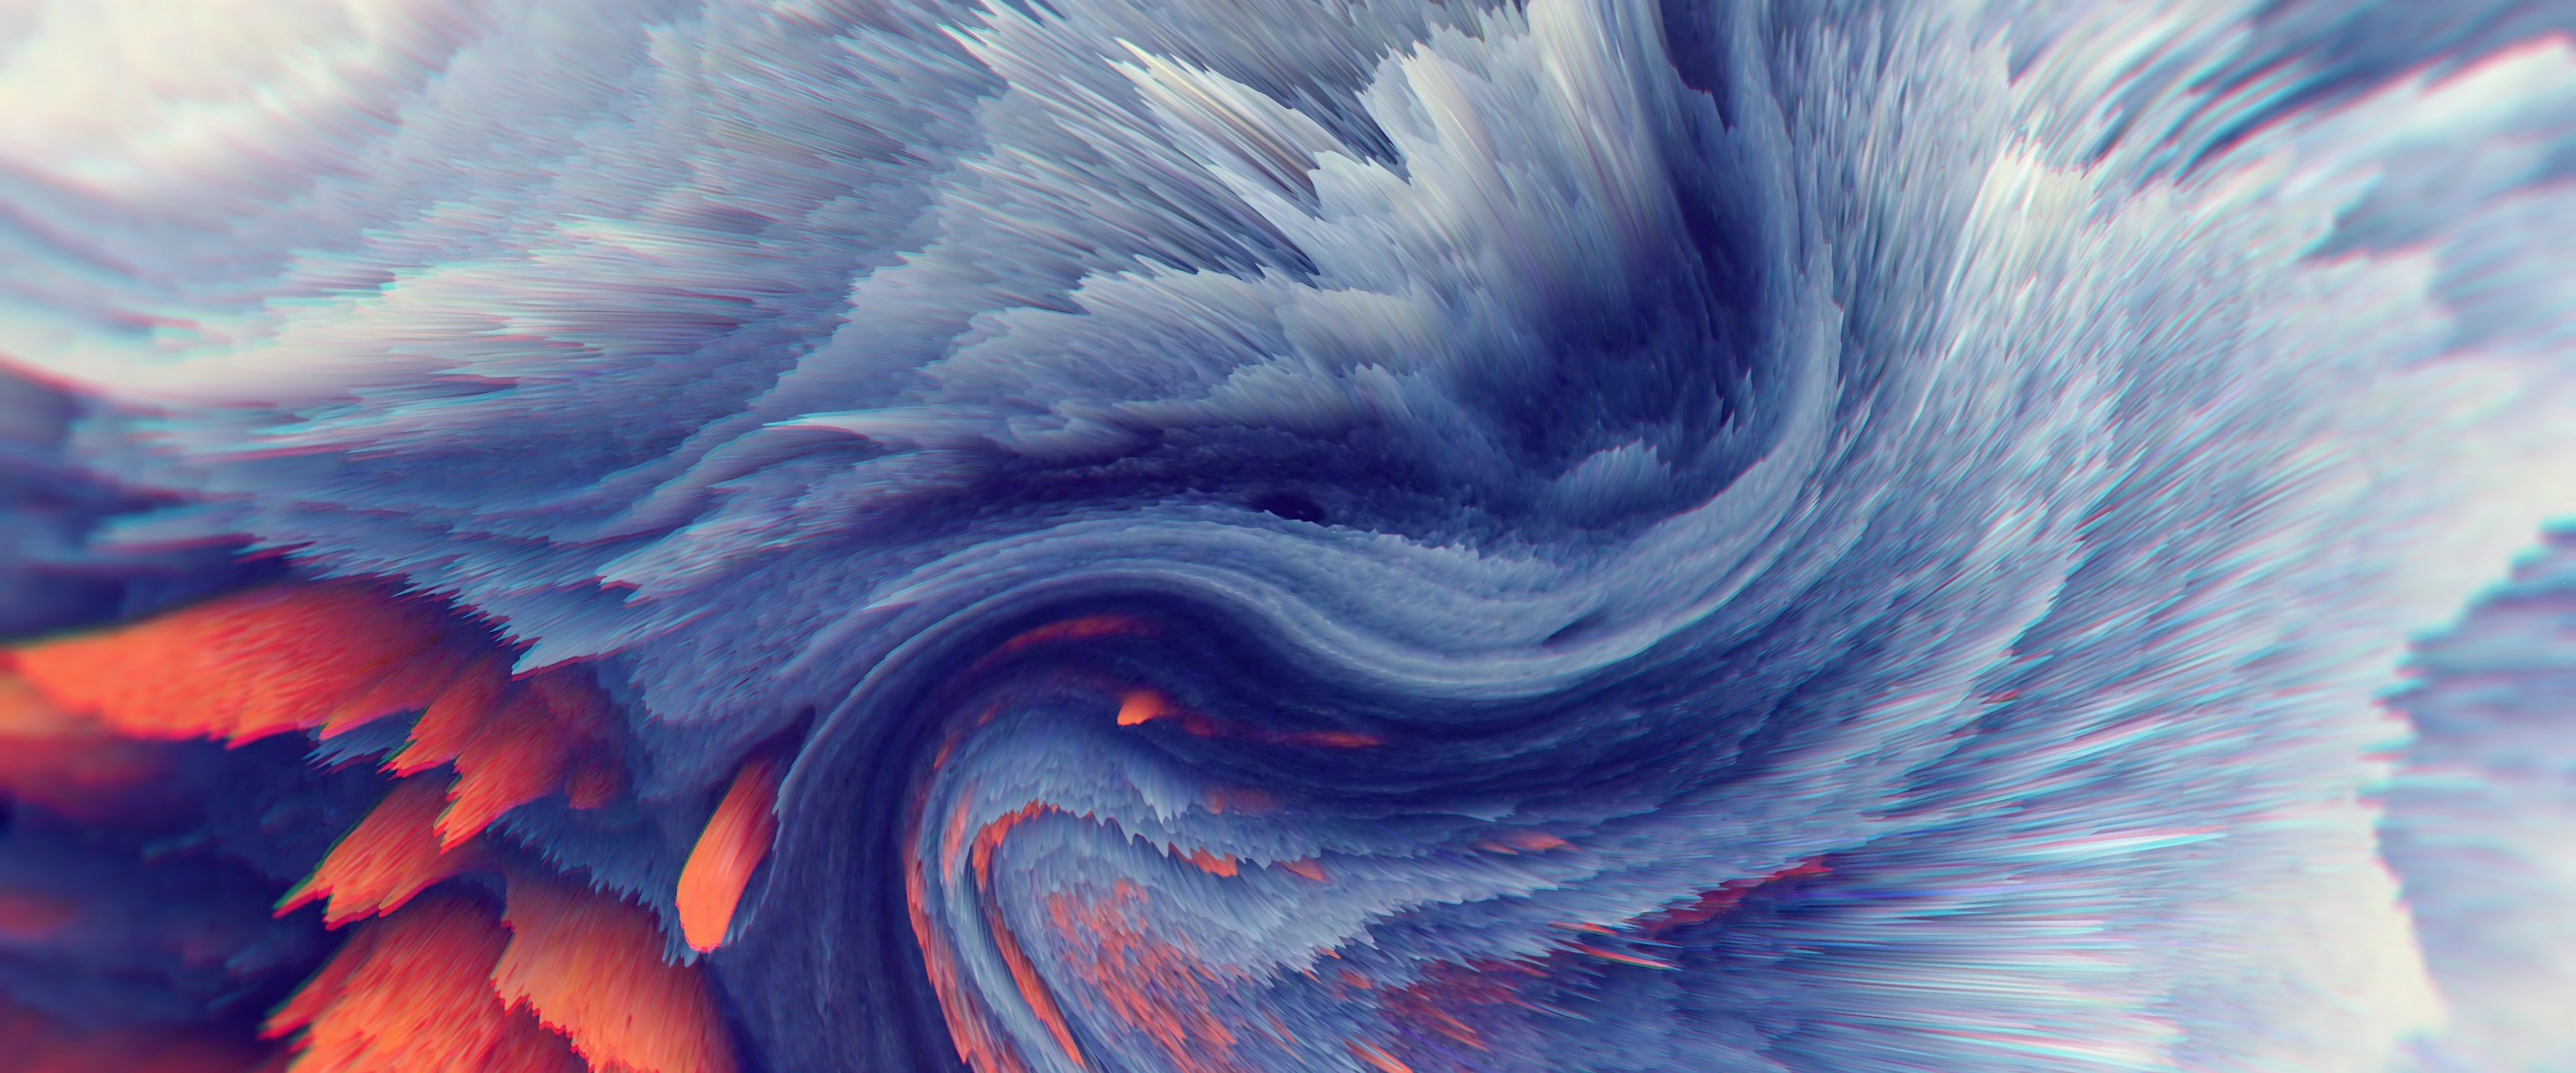
\includegraphics[width=\paperwidth - 4cm, height=\paperheight - 4cm]{resources/images/soundwave.jpg}};
    % Start Text
    \vspace{4cm}

    % the title
    {\newUpperTitleFont\thetitle\par}
    \vspace{1cm}

    % the autors
    {\theauthor\par}
    \vspace{.5cm}

    % date
    {\thedate\par}
    \vspace{5cm}

    % showcase
    %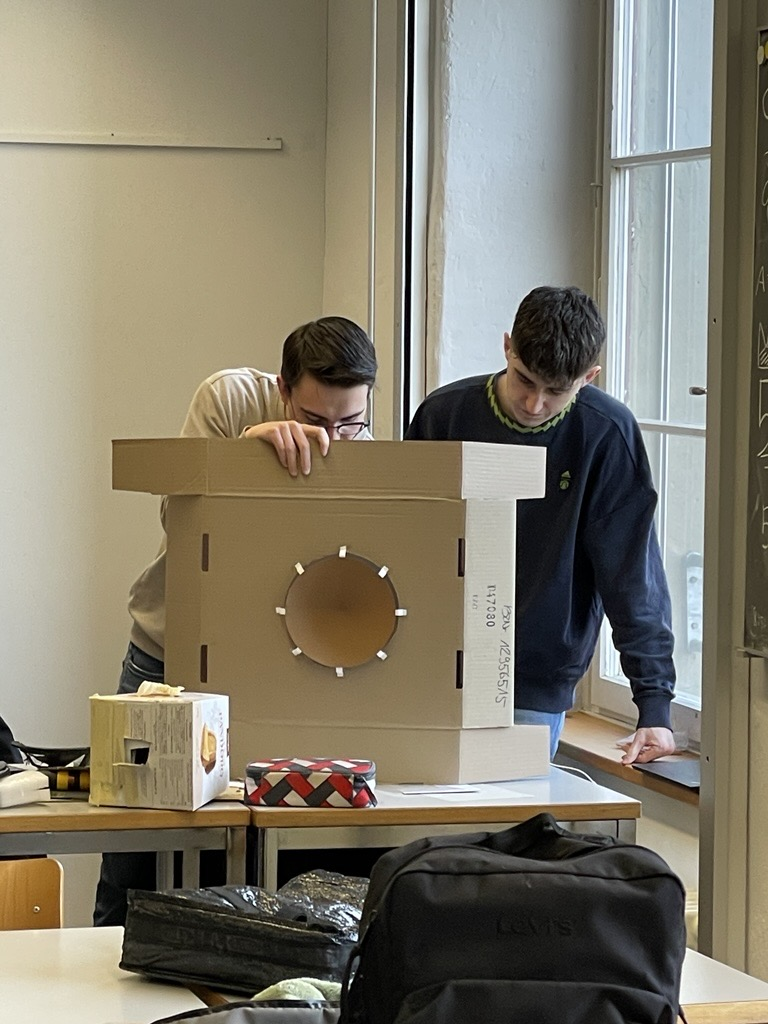
\includegraphics[width=.4\linewidth]{resources/images/Andrin_Cyrill_building.jpeg}
\end{titlepage}

% normal title
%\maketitle

% Abstract
\begin{abstract}
    In dem folgenden Bericht geht es um die Bau eines Lautsprechers aus alltäglichen Materialien.

    Es wurde ein leistungsstarker Lautsprecher gebaut, was vor allem an den starken Magneten liegt.

    Die Bauart aus leichten Materialien für den Schallerzeuger und dem stabilen Klangkörper sorgen für ein gutes Klangerlebnis.
    
\end{abstract}

% Table of contents
\tableofcontents
\thispagestyle{empty}

% report
\pagenumbering{arabic}
\setcounter{page}{1}

% Bericht
\part{Bericht}

% Introduction
\chapter{Einleitung}
\section{Fragestellung}
\begin{enumerate}
    \item Ist es möglich in der Schule einen gut funktionierenden Lautsprecher zu bauen?
    \item Ist es sinvoller einen Magneten innerhalb der Spule oder ausserhalb zu positionieren?
    \item Empfiehlt sich ein dickerer oder dünnerer Draht?
\end{enumerate}
\section{Hypothese}
\begin{enumerate}
    \item Wir gehen davon aus, dass wir einen Lautsprecher bauen können, der bei mittleren Lautstärken funktioniert, aber Schwächen bei sehr lauten Tönen und Bässen hat.
    \item Wir gehen davon aus, dass es sinvoller ist den Magneten ausserhalb der Spule zu positionieren.
    \item Wir gehen davon aus, dass ein dicker Draht sinvoller ist, da er weinger Widerstand hat und somit weniger Wärme erzeugt.
\end{enumerate}

\newpage
\section{Theorie}
\subsection{Wichtige Formeln}
\textbf{Relevante Variablen} \par
\begin{tabbing}
    gamma\quad\= a Greek latter\kill
    \(\mu_0\) :     \> magnetische Permeabilität des Vakuums \\
    \(\mu_r\) :     \>magnetische Permeabilität des Füllmaterials \\
    \(N\) :         \> Anzahl Windungen \\
    \(I\) :         \>Stromstärke \\
    \(L\) :         \>Länge der Spule \\
\end{tabbing}

\textbf{Berechnung der magnetischen Permeabilit im Vakuum}
\begin{equation}
    \mu_0 = 4 \cdot \pi \cdot 10^{-7} \frac{V \cdot s}{A \cdot m}
\end{equation}\par

\textbf{Berechnung der magnetischen Kraft mit Füllmaterial}
\begin{equation}
    B(r) \approx \frac{\mu_0 \cdot \mu_r \cdot N \cdot I}{L}
\end{equation}\par

\subsection{Geschichte des Lautsprechers}

\begin{wrapfigure}{r}{0.4\textwidth}
    \centering
    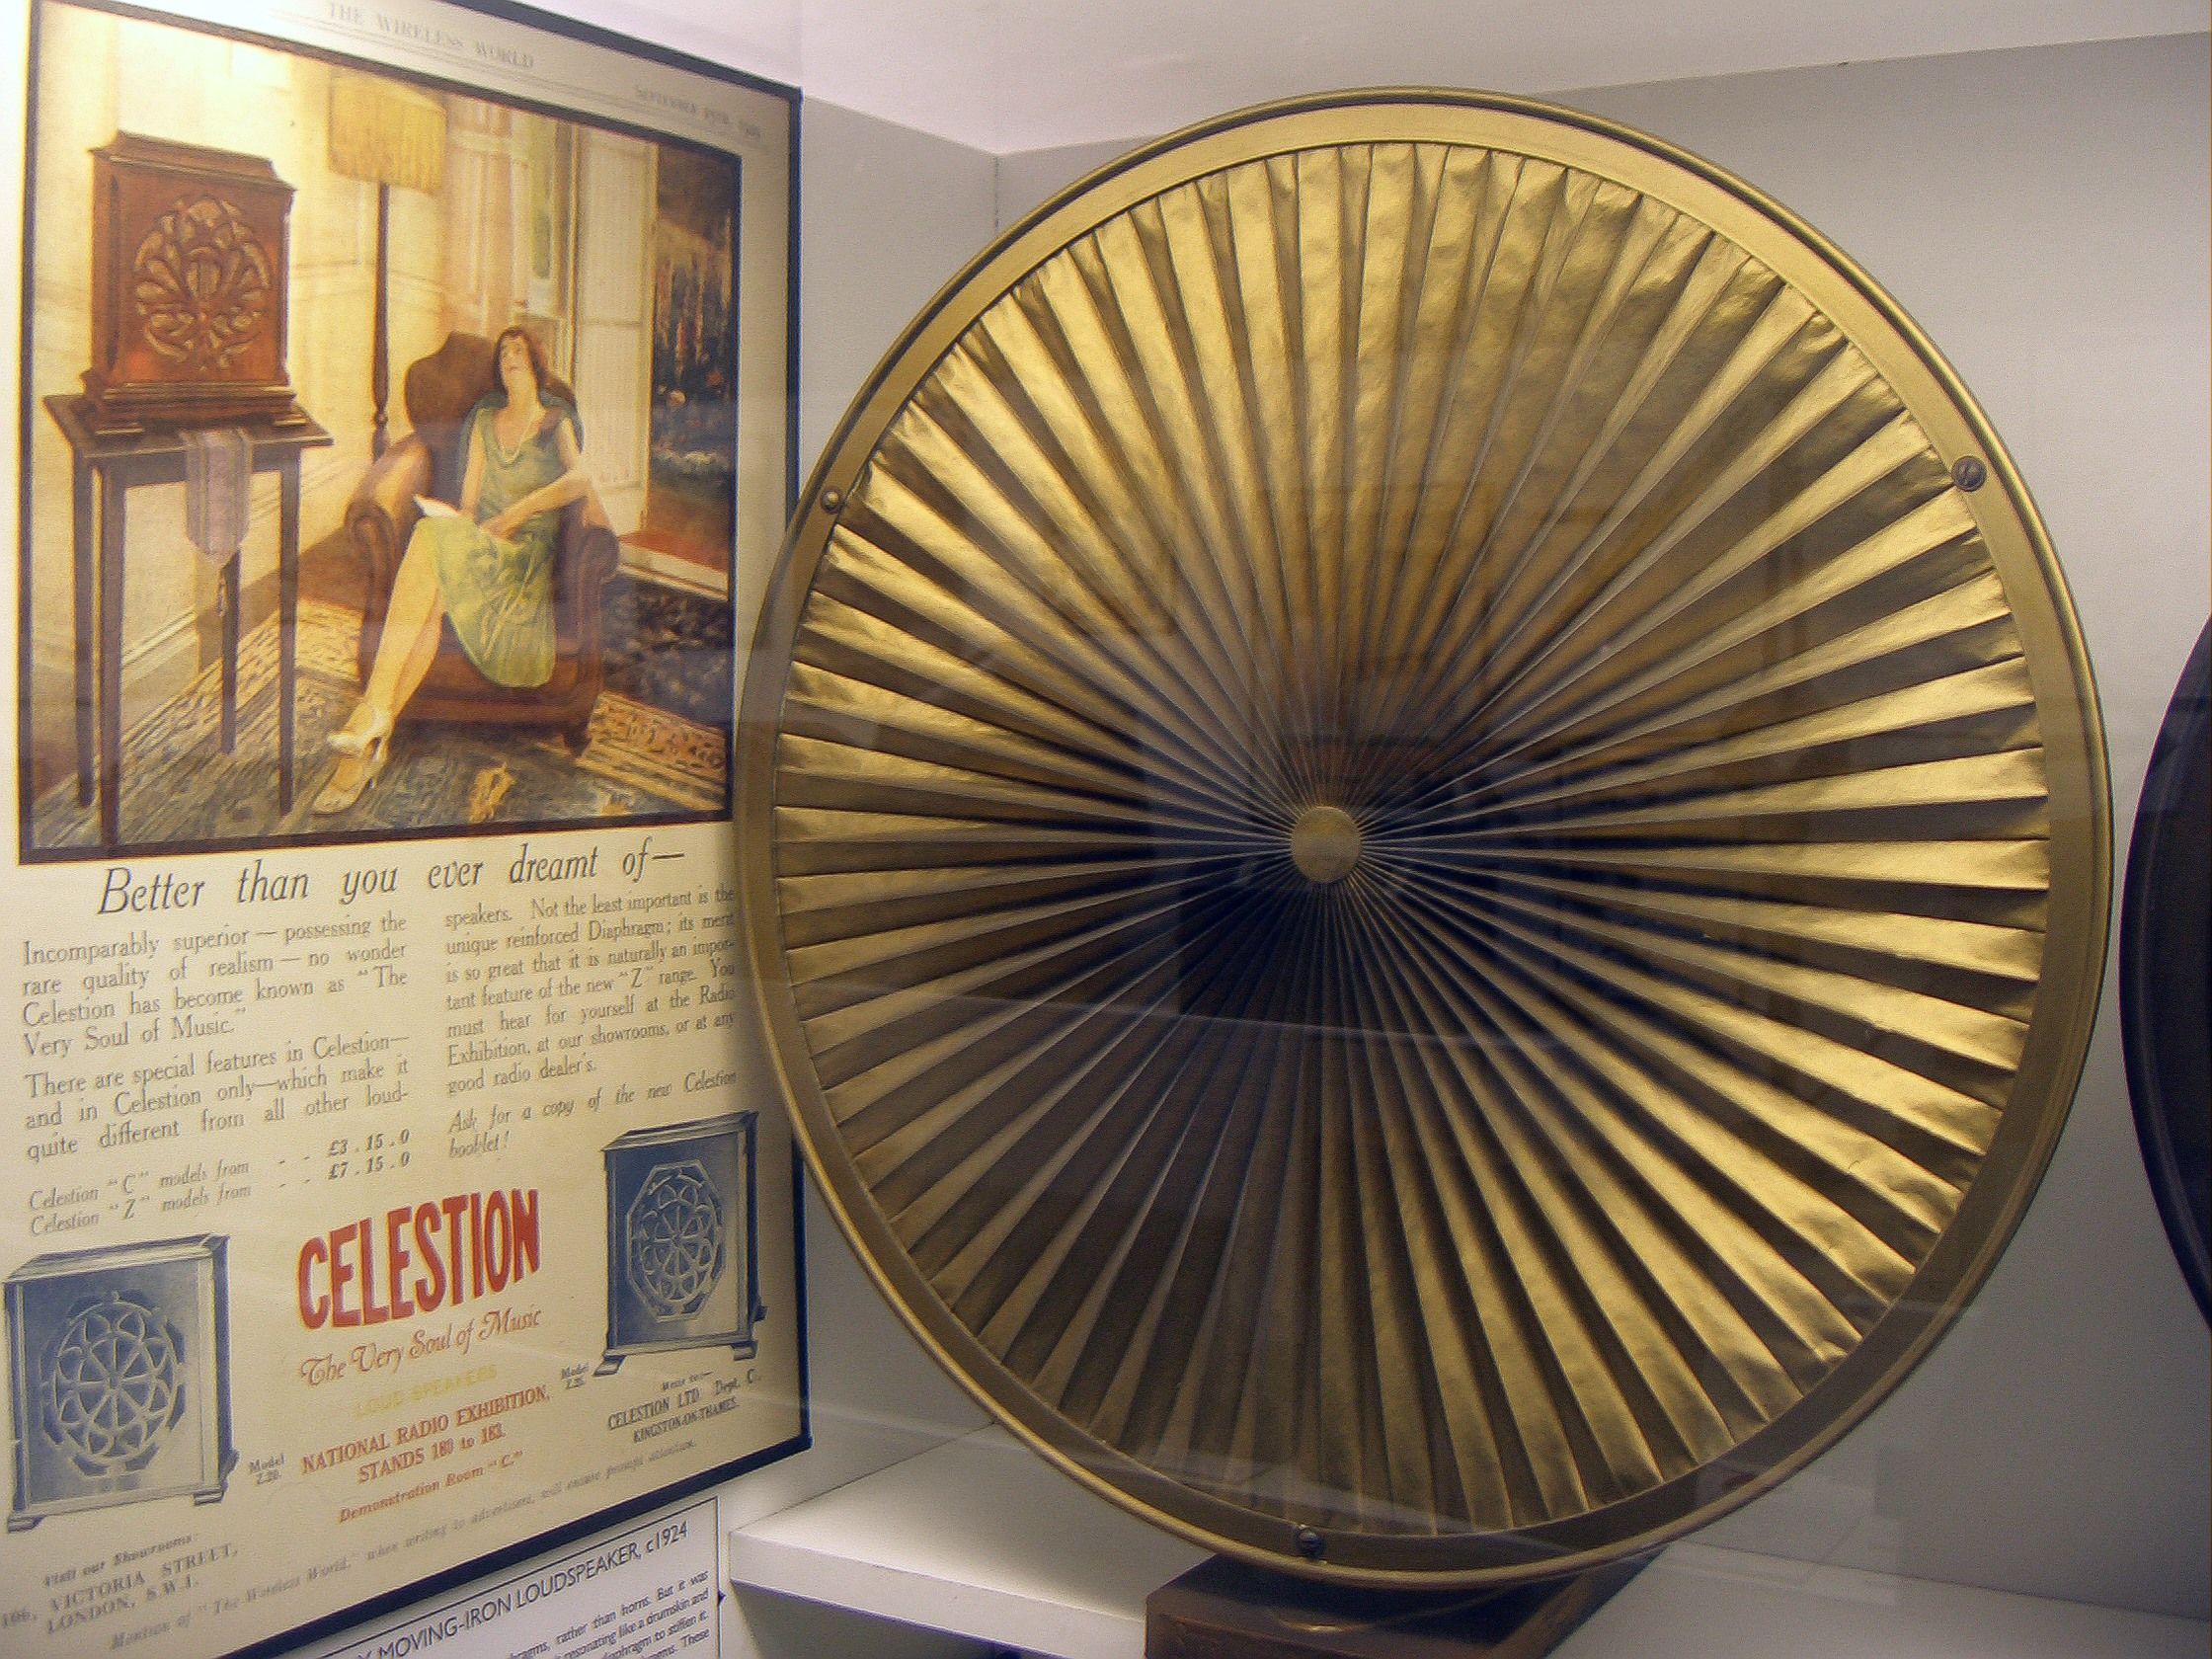
\includegraphics[width=.95\linewidth]{resources/images/Lautsprecher_Celestion.jpg}
    \caption{\raggedright{Lautsprecher von Celestion}}
    \label{fig:celection_speaker}
\end{wrapfigure}

Der Lautsprecher wurde im Jahre 1861 als mechanisches Nebenprodukt des Telefons entwickelt.

1878 wurde dann das Patent zu einem elektrischen Lautsprecher eingereicht, welches letztlich erst 1925 präsentiert wurde.
Das Grundprinzip blieb bis heute unverändert und ist in den Meisten Lautsprechern Vorzufinden. \cite{history_wikipedia}

Aufgrund der damaligen Bauart waren die Lautsprecher meinst sehr gross. Dies war Aufgrund der weichen Einspannung. \cite{history_connect}

Einen Entwickler für den Lautsprecher kann man jedoch nicht genau nennen, da es eine fliessende Entwicklung war, welche zum dem Produkt führten.

Vielen forschten gleichzeitig in diesem Thema und Patente unterschieden sich nur wage. Teils waren die Patente in den USA und Deutschland sogar nahezu identisch.\cite{history_tu_berlin}

% How to build it properly
\newpage
\subsection{Ideale Bauweise}
\subsubsection*{Bassreflexgeäuse}
\vspace{.5cm}
\noindent \begin{minipage}{0.6\textwidth}
    Um eine möglichst guten Bass zu generieren ist die Bauart eines Bassreflex-Gehäuses optimal. Durch die offene Bauweise mit einem sogenannten "Bassrefelexkanal" versehen.
    Das Innere des Körpers wird als Resonator gebraucht, um den Bass zu verstärken.
\end{minipage}
\hspace{0.1\textwidth}
\begin{minipage}{0.2\textwidth}
    \includegraphics[width=.9\textwidth]{resources/images/Bassreflex-Gehäuse.png}
    \captionof{figure}{\raggedright Bassreflex-Gehäuse}
    \label{fig:bass-reflex}
\end{minipage}
\vspace{.5cm}

Dabei wird als allgemeine Formel für die Berechnung der Resonator-Kanälen mit kreisförmigen Querschnitt
\begin{tabbing}
    gamma\quad\= a Greek latter\kill
    d :    \>Durchmesser (in cm) \\
    l :    \>Länge (in cm)
\end{tabbing}

\begin{equation}
    l = \frac{23400 \cdot d^2}{f^2 \cdot V_b} - 0.8 \cdot d
\end{equation}
Dies ist jedoch vor allem für einen reinen Bass gut geeignet.\cite{bassreflex_wikipedia}

\subsubsection*{Frequenzweichen Theorie}
Über eine Frequenzweichen ist es möglich die Frequenz aufzuteilen und somit einen Lautsprecher mit mehreren Membranen zu bauen.

Ein Beispiel wäre einen Hochtöner und einen Tieftöner zu kombinieren. Durch die unterschiedlichen Vorraussetzungen der Bauart der beiden Komponenten, ist dies essentiell um die Frquzenzen zu entfernen, welche durch die jeweilige Membran nicht korrekt dargestellt werden kann.

Das ganze sieht schematisch folgendermassen aus: \\
\begin{center}
    \begin{tikzpicture}[rotate=-90, circuit ee IEC,x=3cm,y=2cm,semithick,
        every info/.style={font=\footnotesize},
        small circuit symbols,
        set resistor graphic=var resistor IEC graphic,
        set diode graphic=var diode IEC graphic,
        set make contact graphic= var make contact IEC graphic]
    % Let us start with some contacts:
    \foreach \contact/\y in {1/1,2/2,3/3.5,4/4.5}
    {
    \node [contact] (left contact \contact) at (0,\y) {};
    \node [contact] (middle contact \contact) at (1,\y) {};
    \node [contact] (right contact \contact) at (2,\y) {};
    }
    \draw (right contact 1) -- (right contact 2) -- (right contact 3)
    -- (right contact 4);
    
    \draw (left contact 1) to ++(down:1)
             to [ac source] ++(right:2)
             to (right contact 1);
    
    \draw (left contact 1) to (left contact 2);
    \draw (left contact 2) to [inductor] (middle contact 2);
    \draw (middle contact 1) to (middle contact 2);
    \draw (middle contact 1) to [capacitor] (right contact 1);
    \draw (middle contact 2) to [resistor={info={[SlateBlue1]$TT$}}] (right contact 2);
    \draw (left contact 2) to (left contact 3);
    \draw (left contact 3) to (left contact 4);
    \draw (left contact 4) to [capacitor] (middle contact 4);
    \draw (middle contact 3) to (middle contact 4);
    \draw (middle contact 3) to [inductor] (right contact 3);
    \draw (middle contact 4) to [resistor={info={[SlateBlue1]$HT$}}] (right contact 4);
    \end{tikzpicture}
\end{center}

% Materials and Methods
\chapter{Material und Methoden}
\section{Material}
Bei den Materialien gab es spezifische Ansprüche an Rubustheit und Hitzebeständigkeit.

Alle Teile, welche um die Spule gebaut wurden, musste auch bei sehr hohen Temperaturn noch intakt bleiben (bis zu 200°C).

Bei den Materialien des Körpers wurde auf eine die Stabilität geachtet und auf die möglichkeit es an den nötigen Stellen gut zu isolieren, damit der Schall nicht schwindet.
\section{Methoden}
Es wurde sehr viel im Internet recherchiert, um herauszufinden wie etwas optimal gebaut werden kann. Zudem versuchte man auch durch ausprobieren, das Optimum aus den zur Verfügung stehenden Materialien zu finden.

Sehr viel wurde im Physiklabor mit grosser Unterstüzung des Laboranten gearbeitet. Zudem wurde zu Hause auch weiter gebaut. Der grösste Aufwand des ganzen war das handwerkliche Bauen des Lautsprechers selbst.

Ebenfalls wurden CAD Programme verwendet, um einen Plan des Ganzen zu erstellen.
\chapter{Resultate}

Platz für alle Bilder des Prozesses

\chapter{Diskussion}

% Baudokumentation
\part{Baudokumentation}

% How to build it
\chapter{Plan}
\section{CAD Zeichnung}
\section{Skizzen}

% How it was built
\chapter{Bau}
\section{beöntigte Materialien}
\begin{multicols}{2}
    \begin{itemize}[parsep=0pt]
        \item Schleifpapier (für Klangerzeuger und Kupferdraht zu endisolieren)
        \item Kupferdraht (0.2mm)
        \item Karton für den Körper der Spule
        \item Bananenkabel
        \item Isolierband
        \item Zähler (für Umwicklungen)
        \item Verstärker
        \item Kartonbox
        \item Schere
        \item Cutter
        \item Multimeter
        \item Taschenmesser
        \item Ofenschnurkleber (bis 1100°C)
        \item Werkzeuge des Physiklabors
        \item Weinkiste
        \item Holzplatte
        \item Schleifpapier
    \end{itemize}
\end{multicols}
\section{Bauanleitung}
\subsection{Gehäuse}
\begin{enumerate}
    \item Eine Weinkiste wurde als Gehäuse für den Lautsprecher selbst werwendet.Es musste eine passende Deckplatte zugeschnitten werden. Um diese zu befestigen wurden Gewindeeinsätze eingebaut, um es einfach an- und abschrauben zu könnenn.
    \item In die Weinkiste wurden Löcher gesägt, die etwas grösser waren als die Membran, damit sie dort Platz finden.
    \item Zwischen die Dickplatte und die Weinkiste wurde ein Dichteband angebracht. Diese isoliert den Klang im Gehäuse und dämpft das Ganze zusätzlich.
    Die Kiste wurde zudem allgemein allgemein an undichten Stellen isoliert. 
\end{enumerate}
\subsection{Tieftönergestell}
\begin{enumerate}
    \item Für die grosse Membran des Tieftöners wurde eine Holzkonstruktion an die Deckplatte gebaut, welche aus 4 Pfeilern besteht, welche diagonal mit Querstreben verbunden sind.
\end{enumerate}
\subsection{Tieftöner}
\begin{enumerate}
    \item
\end{enumerate}
\subsection{Hochtöner}
\begin{enumerate}
    \item 
\end{enumerate}

% Tanking
\chapter*{Dank}
Ein grosser Dank geht an den Physiklehrer Patrick Perucchi, welcher uns regelmässig mit Tipps und Tricks zur optimierung der Bauweise unterstützt hat.
Ein weiterer Dank geht an Herrn Daniel Meyer, welcher uns bei den Berechnungen der Frequenzweiche mit seiner Erfahrung unterstützen konnte, sowie an Markus Lerjen, welcher uns bei der Optimierung derer unterstützt hat.

Ebenfalls bedanken wir uns beim Pyhsiklaboranten und Sprengmeister Herrn Mohammed Zumsteg, welcher uns in der Werkstatt stehts zur Seite stand, uns einen Teil der Materialien und Werkzeuge zur Verfügung stelle und immer gute Sprüche geklopft hat.



% List of figures
\newpage
\listoffigures

% Sources
\newpage
\bibliographystyle{plain}
\bibliography{mybib}
\end{document}